\documentclass{article}
\usepackage{float}
\usepackage{graphicx}
\renewcommand{\baselinestretch}{1}
\setlength{\textheight}{9in}
\setlength{\textwidth}{6.5in}
\setlength{\headheight}{0in}
\setlength{\headsep}{0in}
\setlength{\topmargin}{0in}
\setlength{\oddsidemargin}{0in}
\setlength{\evensidemargin}{0in}
\setlength{\parindent}{.3in}
\newtheorem{hypothesis}{Hypothesis}
\newtheorem{nullhypothesis}{Null Hypothesis}
\begin{document}

\section{Evaluation}

\subsection{Statistics}

The annotation table obtained from the image labelling is in the form of rectangle location and dimensions of the bounding box dimensions. The datasets are divided into three sets
\begin{enumerate}
\item \textit{Training Dataset}: annotation data obtained using the consumer drone and used for training the model.
\item \textit{Testing Dataset}: annotation data obtained using the consumer drone and used for testing the model.
\item \textit{GeoScience Dataset}: annotation data obtained using the data obtained from the GeoScience Department using a commercial drone.
\end{enumerate}

Bounding box heights, widths and aspect ratios can be obtained from the annotation data. The testing data and GeoScience data will be tested against the training data to see whether they are from the same population. If any populations are the same, the analysis done on one population should have the same evaluation results. If the populations are different, the analysis on both will be different, and the algorithms would need to be adapted to cater for this difference.

\subsubsection{Training Dataset}

Training bound boxes have a similar average width and average height pixel sizes. The average size is around 76 pixels, with minimum pixel size of around 28 pixels. The smallest bounding box matches the $32x32$ VGG16 pixel field of view within the \textit{conv5} output feature map. The highest number of bounding boxes fall under a $2x2$ VGG16 feature map.

\begin{table}[ht]
\caption{Consumer Drone Bounding Box Statistics - Train data}
\centering
\begin{tabular}{llllll}
       & Mean   & Std. Dev. & Min & Max & Population \\
Width  & 73.848 & 28.359 & 25 & 206  & 524 \\
Height & 79.293 & 27.197 & 31 & 207  & 524
\end{tabular}
\end{table}

\begin{figure}[h]
\centering
\label{consumerdronetrainhist}
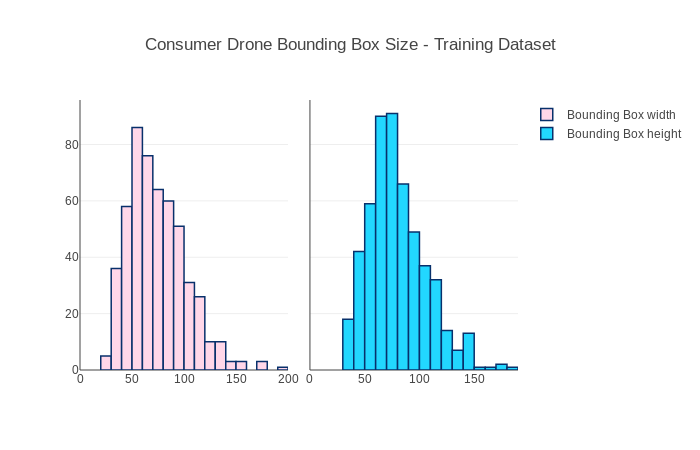
\includegraphics[scale=0.4]{images/train-histogram.png}
\caption{Consumer Drone Bounding Box Height and Width Histograms- Train data}
\end{figure}

As per qqplot show in figure \ref{consumerdronetrainqqplot} the data does not follow a normal distribution, so non-parametric tests will be performed to check that samples are obtained from the same population. 

\begin{figure}[h]
\centering
\label{consumerdronetrainqqplot}
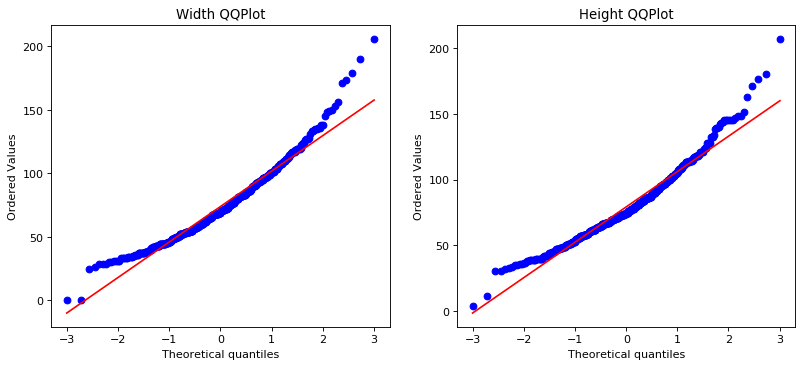
\includegraphics[scale=0.4]{images/train-qqplot.png}
\caption{Consumer Drone Bounding Box Height and Width QQplot - Train data}
\end{figure}

The aspect ratio of the training set as shown in the figure \ref{consumerdronetrainaspect} shows that there is no preference between log(-0.5) to log(0.5). This shows that there is no orientation preference of the bounding boxes in the training data set. As can be expected from aerial imagery data.

\begin{figure}[h]
\centering
\label{consumerdronetrainaspect}
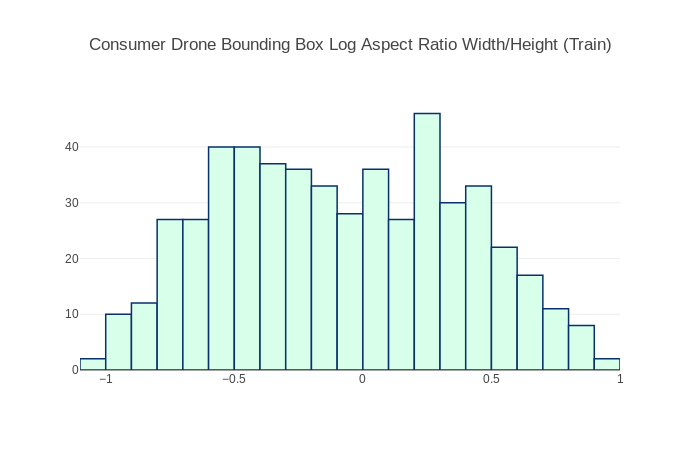
\includegraphics[scale=0.4]{images/train-aspect.png}
\caption{Consumer Drone Bounding Box Log Aspect Ratio Histogram - Train data}
\end{figure}

\subsubsection{Testing Dataset}

Testing bound boxes have a minor tendency to be larger in height than in width. The average size is also around 76 pixels, with minimum pixel size of around 29 pixels. Again this is within the field of view of the VGG16 pixel single feature vector of the \textit{conv5} output feature map. 

\begin{table}[ht]
\caption{Consumer Drone Bounding Box Statistics - Test data}
\centering
\begin{tabular}{llllll}
       & Mean   & Std. Dev. & Min & Max & Population\\
Width  & 71.654 & 29.435 & 26 & 199 & 246 \\
Height & 81.232 & 34.203 & 30 & 272 & 246
\end{tabular}
\end{table}

\begin{figure}[h]
\centering
\label{consumerdronetesthist}
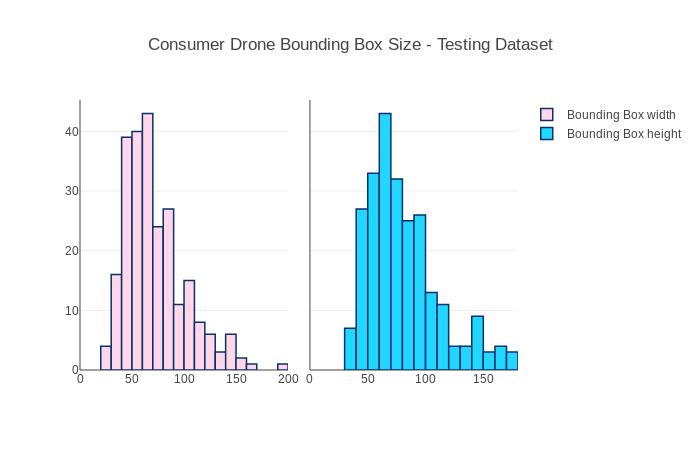
\includegraphics[scale=0.4]{images/test-histogram.png}
\caption{Consumer Drone Bounding Box Height and Width Histograms- Test data}
\end{figure}

As per qqplot show in figure \ref{consumerdronetrainqqplot} the data does not follow a normal distribution. This confirms the non-parametric tests to be performed on the population sampling.

\begin{figure}[h]
\centering
\label{consumerdronetestqqplot}
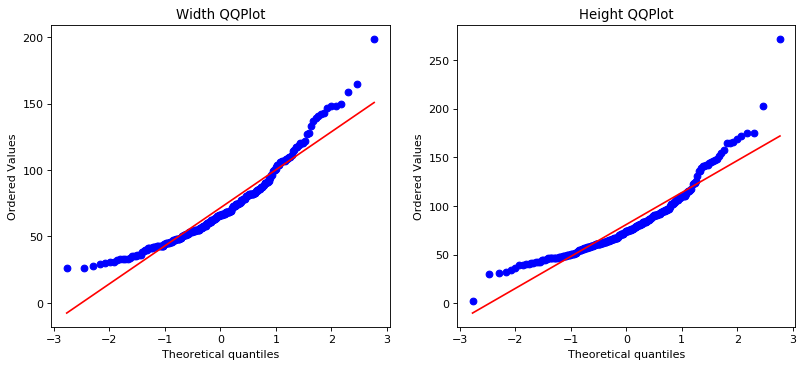
\includegraphics[scale=0.4]{images/test-qqplot.png}
\caption{Consumer Drone Bounding Box Height and Width QQplot - Test data}
\end{figure}

The aspect ratio of the training set as shown in the figure \ref{consumerdronetrainaspect} shows that there is no preference between log(-0.5) to log(0.5). This shows that there is no orientation preference of the bounding boxes in the training data set. The smaller values at the O for both the training set and the test set indicate that the objects bounding boxes are rarely a box shape (i.e. equal width and height) which indicates that the objects have an elongated shape. This is to be expected as the images labelled are of beverage bottles and containers, which are predominantly manufactured to be stacked side-by-side, and ergonomically designed to be handled by a single hand.

\begin{figure}[H]
\centering
\label{consumerdronetestaspect}
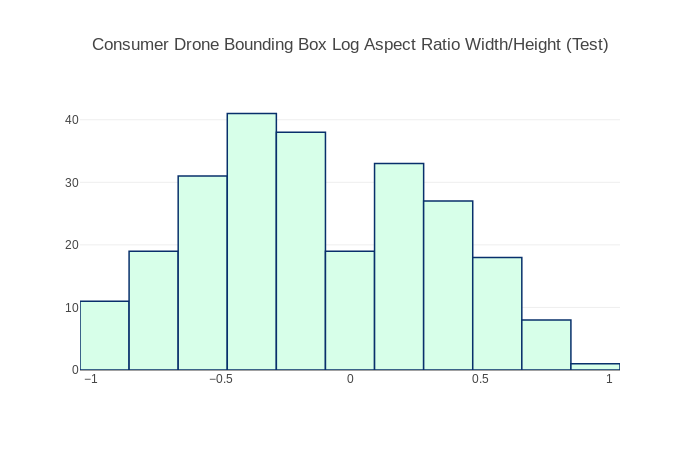
\includegraphics[scale=0.4]{images/test-aspect.png}
\caption{Consumer Drone Bounding Box Log Aspect Ratio Histogram - Test data}
\end{figure}


\subsubsection{GeoScience Dataset}

The Geoscience annotation also show no orientation prefernce with equal average width and height. The average size is also around 37 pixels, with minimum pixel size of around 11 pixels. This is a marked distinction from the previous datasets. The smaller bounding box sizes within this dataset might cause difficulties in the VGG16 field of view.

\begin{table}[ht]
\caption{GeoScience Drone Bounding Box Statistics - Data}
\centering
\begin{tabular}{llllll}
       & Mean   & Std. Dev. & Min & Max & Population\\
Width  & 36.038 & 11.921 & 11 & 120 & 793 \\
Height & 37.318 & 10.420 & 10 & 82 & 793
\end{tabular}
\end{table}

The average size of the bounding boxes of the GeoSciences is half that of the two other datasets. 

\begin{figure}[ht]
\centering
\label{geodronethist}
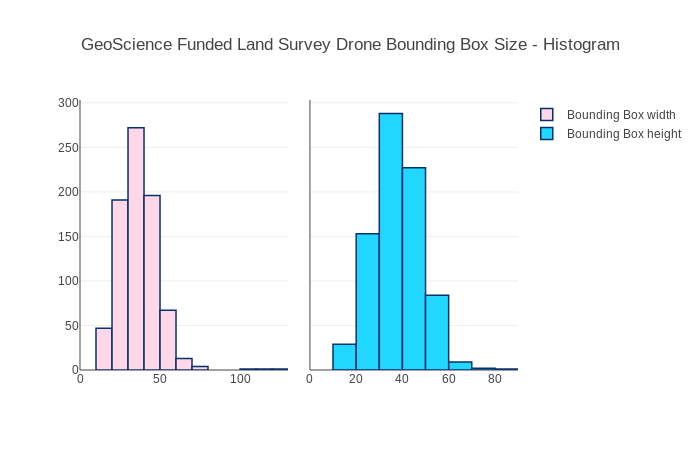
\includegraphics[scale=0.4]{images/geoscience-histogram.png}
\caption{GeoScience Bounding Box Height and Width Histograms}
\end{figure}

As per qqplot show in figure \ref{geodroneqqplot} the data does not follow a normal distribution. This confirms the non-parametric tests to be performed on the population sampling.

\begin{figure}[h]
\centering
\label{geodroneqqplot}
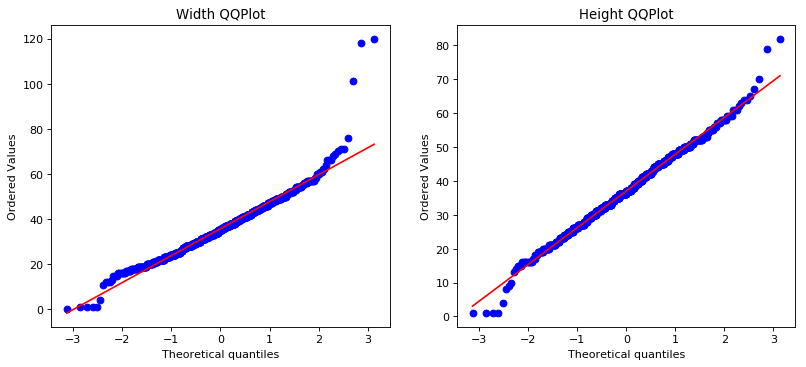
\includegraphics[scale=0.4]{images/geoscience-qqplot.png}
\caption{GeoScience Bounding Box Height and Width QQplot}
\end{figure}

The aspect ratio figure \ref{geodroneaspect} has a similar shape as the train and data set, confirming the nature of the images being labelled. 

\begin{figure}[ht]
\centering
\label{geodroneaspect}
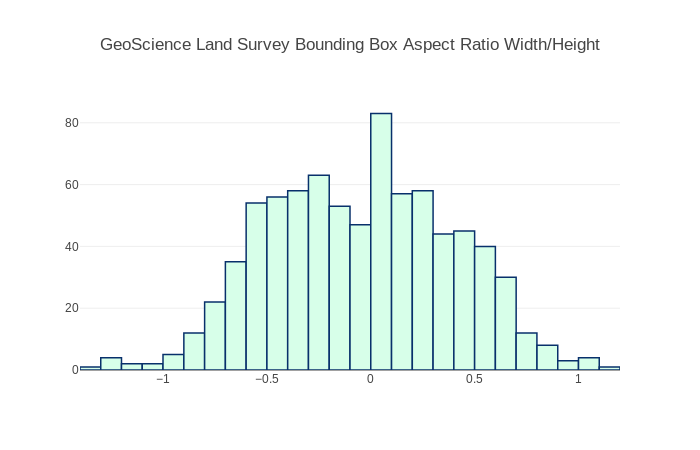
\includegraphics[scale=0.4]{images/geoscience-aspect.png}
\caption{GeoScience Bounding Box Log Aspect Ratio Histogram}
\end{figure}

\subsubsection{Population Testing}

The train, test and Geoscience population will be tested for independance. Since the populations are not normally distrbuted, a non-parametric test will be used. A two-tail Mann Whitney test will be performed. The whole data in the datasets will be used. The scale will be in pixel size. A confidence interval $\alpha = 0.05$ will be used.

The null hypothesis will be formulated :
\begin{nullhypothesis}
$H_0$: the distribution of the pixel sizes of the two datasets are equal
\end{nullhypothesis}
\begin{hypothesis}
$H_{A}$: the distribution of the pixel sizes is not equal
\end{hypothesis}

The two comparisons will be made between train vs test and train vs geoscience dataset.

\subsubsection{Train vs Testing Population}

Testing the two datasets using Mann Whitney results with U = 69299.00 and a p-value of 0.092 (for width) and U = 66246.50 and a p-value of 0.533 (for height) . Therefore we fail to reject the Null Hypothesis $H_0$. The train and testing data set come from the same population. This is to be expected as the data comes from the same sensor and using the same land-survey techniques.

\subsubsection{Train vs GeoScience Population}

Testing the two datasets using Mann Whitney results with U = 383029.00 and a p-value of 0.0 (for width) and U = 400391.50 and a p-value of 0.0 (for height) . Therefore we reject the Null Hypothesis $H_0$. The train and geoscience dataset come from the different populations. 

\subsubsection{Statistical Results}

The statistical tests show that the geoscience and the consumer drone data have different image sizes. This shows that the surveying techniques and parameters are different between geoscience data and consumer drone data. Comparing the geoscience images to that of the consumer drone, it can be deduced that the altitude of the surveys are different. This can also be the result of the drone operator knowledge of higher camera resolution.\newline

An algorithm which is dependant on the size of the picture for successful recognition, will have difficulty correctly infering the smaller sized dataset. The ability of the human labeller to correctly label the objects, indicates that the shape information is present. This has to be exploited by the CNN. The algorithm must be scale invariant or specifically tuned to the zoom levels of the geoscience dataset.\newline

\subsection{CNN Algorithm Testing}

Four CNN architectures will be testing for maximum validation accuracy results. The one with highest validation accuracy and highest Litter recall will be chosen. Each algorithm will be tested pre-trained with Imagenet weights. The fully connected layer at the end of the convolutional layers will be stripped off, and replaced by
\begin{enumerate}
\item A connected layer with softmax activation,
\item A connected layer with relu activation and a connected layer with softmax activation,
\item Two connected layers with relu activation and a connected layer with softmax activation
\end{enumerate}

The connected layer with softmax activation will two class output. The connection layer between the Convolutional Layer and the Fully Connected Layer will be chosen from a Flatten layer, a Max Pooling Layer and a Global Average Pooling Layer. The testing will use the default layer used in the algorithm Imagenet training. If the training procedure does not converge, other layers will be tested.\newline

At this stage the trainable layers will be reserved only for the new fully connected layers. The best algorithm setup will be chosen. Further algorithm tuning will be performed by allowing more layers inside the convolutional blocks to be trained. Incremental training will be performed on previous trained models. An epoch length of 60 will be used for testing. \newline

\subsubsection{Dataset Preparation}

One dataset will be compiled for all tests.

The data will be fed using Keras ImageGenerator with inbuilt data augmentation algorithms. The options used for testing are as follows:
\begin{enumerate}
\item Preprocessing Function: Keras provides algorithm specific preprocessing functions that transform an image to an output tensor of the same shape,
\item Shear range 0.2 : Angle of shear in degrees,
\item Horizontal Flip : Random horizontal flip of image,
\item Verticial Flip: Random vertical flip of image,
\item Zoom Range 0.2: Random zoom between 0.8 and 1.2 of the image size.
\end{enumerate}

All algorithms will have a default input tensor size of $224 x 224$.
The fill-mode parameter is set to true so that no black areas appear within the image. Later RCNN tuning will test more data augment parameters and parameter ranges. \newline

Validation will only be processed. No augmentation of this set is performed.\newline


Training Batch size : 150
Validation Batch size: 50

\subsubsection{Gradient Descent Optimizers}

RMSProp will be used for all the tests. The learning rate will be tuned according to the training and validation convergence speed. Convergence rate varies between 1e-4 to 1e-6.


\subsection{Algorithm Test Results}

\subsubsection{Inceptionv3}


\begin{enumerate}

\item: Inception with Max Pooling Layer, FCN 1-layer 1024 and Softmax Classifier


\begin{figure}[H]
\centering
\label{fig:incv3-sm}
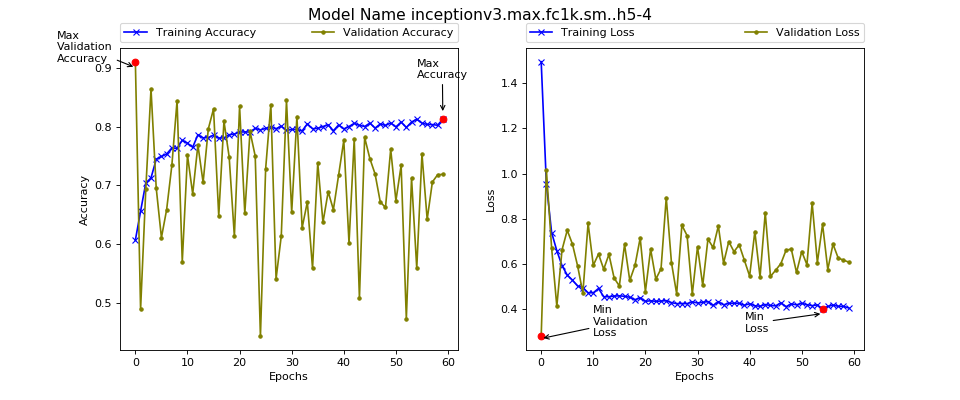
\includegraphics[scale=0.6]{images/t1-i3-fc1k-sm-4.png}
\caption{Inception Training Tasks Max Pooling Layer, FCN 1-layer 1024 and Softmax Classifier}
\end{figure}

The training procedure shows erratic validation training. Validation Accuracy immediately falls from the first epoch validation accuracy of 0.91. Learning rate is 1e-4, which could be too high for convergence. An average accuracy of value of 0.7 is acheived. The MaxPool layer shows a very erratic validation curve, whilst training curve increases gradually to a limit of 0.8. The MaxPooling layer will be dismissed.

\item: Inception with Global AveragePooling Layer and SoftMax Classifier
\begin{figure}[H]
\centering
\label{fig:incv3-gap-4}
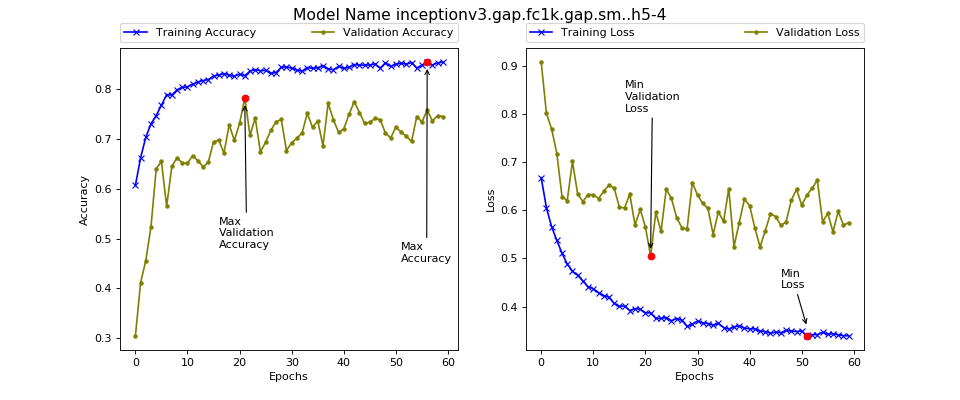
\includegraphics[scale=0.6]{images/t1-i3-gap-sm-4.png}
\caption{Inception Training Tasks GAP and Softmax Classifier - training Softmax layer}
\end{figure}

The InceptionV3 GAP layer maximum validation accuracy acheived when training on 4 layers, is of 0.781 accuracy at epoch 21. The number of trainable layers are increased to 37 layers, whilst using the same weights acheived earlier on. 

\begin{figure}[H]
\centering
\label{fig:incv3-gap-37}
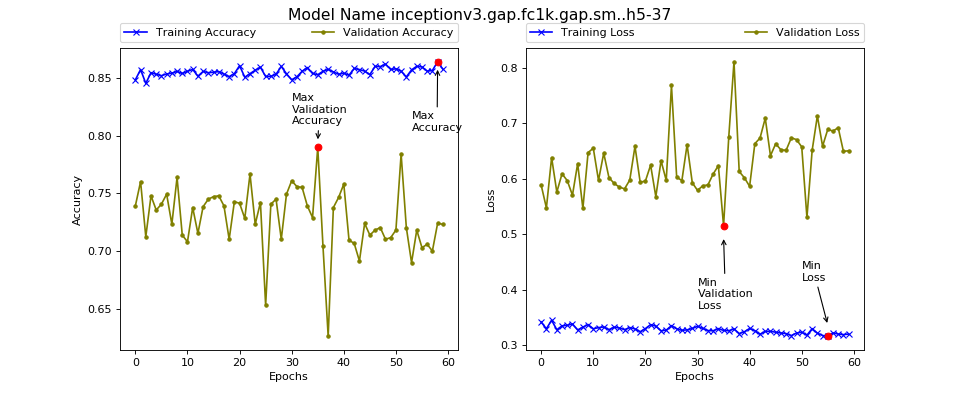
\includegraphics[scale=0.6]{images/t1-i3-gap-sm-37.png}
\caption{Inception Training Tasks GAP and Softmax Classifier - training last 37 layers}
\end{figure}

Validation accuracy increased to 0.79 at epoch 58. The number of trainable layers are increased to 37 layers.

\begin{figure}[H]
\centering
\label{fig:incv3-gap-4}
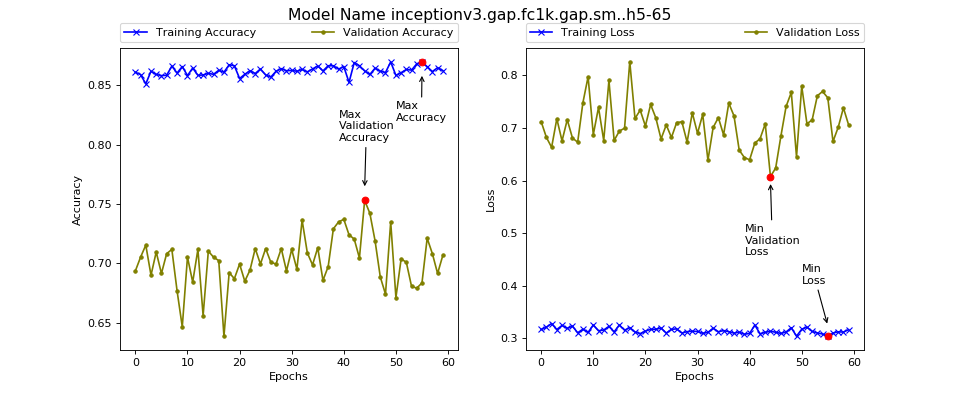
\includegraphics[scale=0.6]{images/t1-i3-gap-sm-65.png}
\caption{Inception Training Tasks GAP and Softmax Classifier - training last 65 layers}
\end{figure}

No further increase in accuracy has been noted, and the validation accuracy levels off at 0.7 mark average. To note the gradual improvement in training accuracy levels, during the training procedure , however the validation is more erratic. This shows a direct neural network to the convolutional output is unable to obtain the classifier features directly. The training accuracy levels off at a 0.87 mark, showing no increase during the last 120 epochs of the total 180 epochs run using a Global Average Pooling Layer. 

\end{enumerate}
\subsubsection{Resnet-50}



\subsubsection{MobileNetv2}

A successful mobilenetv2 implementation will help us increase the speed of all subsequent inferencing. The default depth multiplier of 1 and default number of filters in the layer will be used as per paper. 

Two connection layers will be used Flatten and GlobalAveragePooling layer.

\begin{enumerate}
\item Mobilenet with Flatten Layer and Softmax Classifier 

Maximum Validation accuracy of 0.944 acheived at epoch 53. Training curve is gradual, whilst validation curve is constant with single degredatation points.

\begin{figure}[H]
\centering
\label{fig:mob3-1}
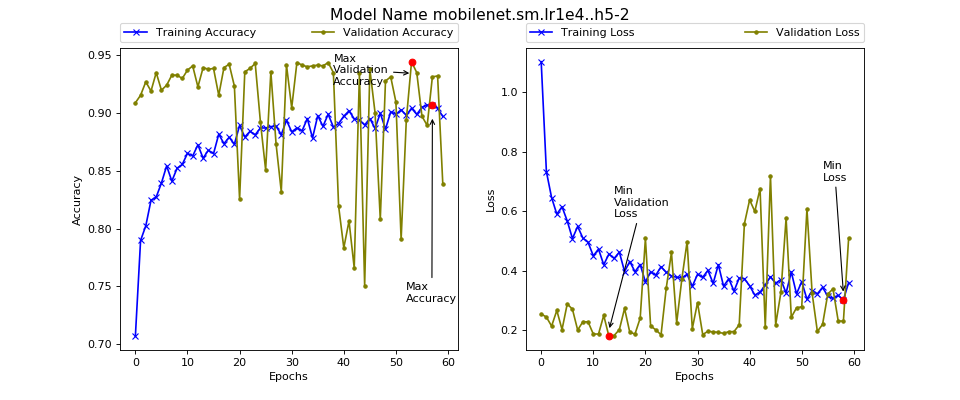
\includegraphics[scale=0.6]{images/mob3-1.png}
\caption{MobileNetv3 Training Flatten and Softmax Classifier - training Softmax only}
\end{figure}

Incremental training on previous architecture using 13 trainable layers. The maximum validation accuracy increased to 0.966. The validation accuracy is not incrementing, showing an overfitting of the training data. Training accuracy has a gradual increase from training epoch 40 onwards.

\begin{figure}[H]
\centering
\label{fig:mob3-2}
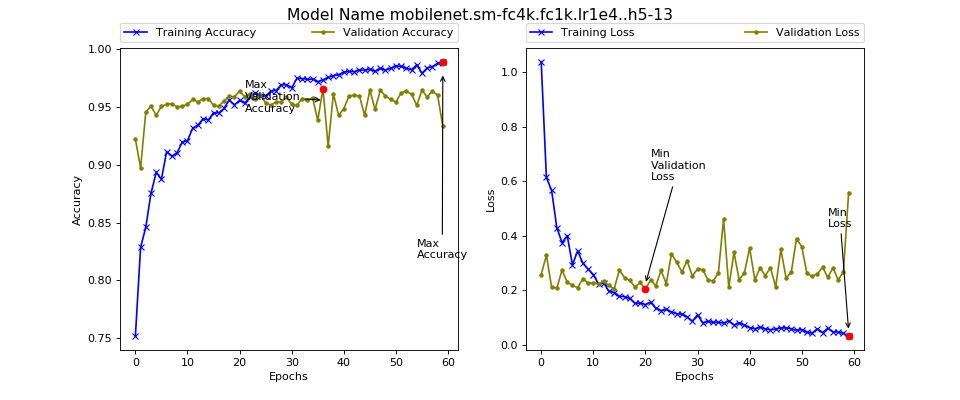
\includegraphics[scale=0.6]{images/mob3-2.png}
\caption{MobileNetv3 Training Flatten and Softmax Classifier - training 13 layers}
\end{figure}

A maximum validation accuracy of 0.987 is seen, where the curve is seen to level off. 

\begin{figure}[H]
\centering
\label{fig:mob3-3}
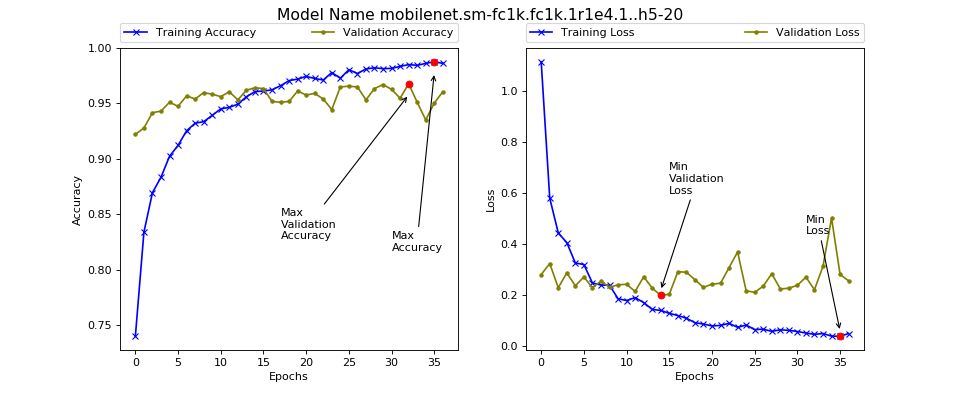
\includegraphics[scale=0.6]{images/mob3-3.png}
\caption{MobileNetv3 Training Flatten and Softmax Classifier - training 20 layers}
\end{figure}


\end{enumerate}


\subsubsection{VGG-16}

\end{document}

